\documentclass{standalone}

\usepackage{tikz}


\begin{document}
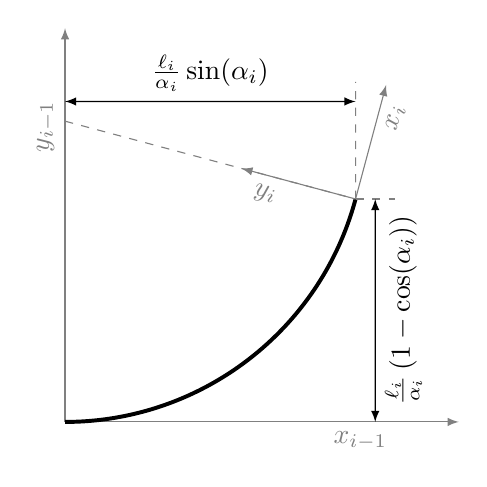
\begin{tikzpicture}[
	scale=5,
	axis/.style={gray},
	dut/.style={line width=.5mm},
	helpline/.style={gray, dashed},
	distarrow/.style={latex-latex}
	]

\def\l{1}
\def\alp{75}

\pgfmathsetmacro{\R}{180*\l/3.14159/\alp}



\draw[-latex, axis] (0,0)--++(1,0)node[below, near end]{$x_{i-1}$};
\draw[-latex, axis] (0,0)--++(0,1)node[sloped, above, near end]{$y_{i-1}$};

\draw[dut] (0,0)arc(-90:-90+\alp:\R)coordinate(X);

\draw[helpline] (0,\R)--(X);
\path(0,\R+.05)-|(X) coordinate[pos=.5] (help);
\draw[helpline] (X)--(help)--++(0,.05);

\draw[distarrow] (0,\R+.05)--(help)node[midway, above]{$\frac{\ell_i}{\alpha_i}\sin(\alpha_i)$};


\path(0,0)-|(X) coordinate[pos=.5] (help);
\path(help)++(.05,0)coordinate(help);
\draw[helpline] (X)--++(.05,0)coordinate(help_)--++(.05,0);
\draw[distarrow] (help_)--(help) node[sloped, midway, below]{$\frac{\ell_i}{\alpha_i}\left(1-\cos(\alpha_i)\right)$};



\draw[-latex, axis] (X)--++(\alp:.3)node[sloped,below, near end]{$x_{i}$};
\draw[-latex, axis] (X)--++(90+\alp:.3)node[sloped, below, near end]{$y_{i}$};



\end{tikzpicture}
\end{document}